\section{Discussion}\label{sec:discussions}

First comprehensive analysis of Sgr A* including both resolved VLBI data and multiwavelength data.

Discussion organized according to physical parameters of the model.

\note{Avoid figures where possible.}

%==============================================================================
\subsection{MAD, SANE, and Self-Consistent Wind Feeding}

\note{Angelo to provide first draft}

There are clear differences between MAD and SANE models in VLBI data, as well as in the non-VLBI data.

Assessment of Ressler model.  Viable!

%==============================================================================
\subsection{Electron Distribution Function}

\note{Koushik to provide first draft}

Strong constraint on abundance of cold electrons from bremss.  A high density of cold electrons - which would be invisible in synchrotron - are ruled out.  This is in part because at $\Theta_e \equiv k T_e/(m_e c^2) \lesssim 1$, $j_\nu \propto \Theta_e^{-1/2}$ (emission in the x-ray band increases as temperature decreases).  In contrast, for $\Theta_e \gtrsim 1$ electron-electron bremsstrahlung becomes important and $j_\nu \propto \Theta_e^{+1/2}$.

Strong constraint on abundance of hot electrons from NIR.  In particular for

Strong constraint on $T_i/T_e$: models with ion temperature equal to electron temperature fail on several counts.

%==============================================================================
\subsection{Inclination}

\note{Michi to provide first draft}
\note{Strong constraints on inclination from m-ring fitting.}

...

%==============================================================================
\subsection{Position Angle}

\note{Virtually no constraint on position angle [check m-ring fits]}

...

%==============================================================================
\subsection{Black Hole Spin}

\note{Still quite weak constraints on black hole spin.}

...

%==============================================================================
\subsection{Accretion Rate and Outflow Power}

\note{Vedant to provide first draft of thermal section.}

Linear polarization and Faraday rotation measurements of \sgra at millimeter and submillimeter wavelengths (\citealt{2000ApJ...538L.121A, 2000ApJ...545..842Q, 2003ApJ...588..331B, 2006ApJ...640..308M, 2006JPhCS..54..354M, 2006ApJ...646L.111M}) and X-ray emission  (\citealt{2003ApJ...591..891B, doi:10.1126/science.1240755}), in conjunction with semi-analytic models estimate the accretion rate $\dot{M}$ as $10^{-9}$ to $10^{-7} M_{\odot}$yr$^{-1}$. The broad range of values is due to the differences in regions of radio emission in the theoretical models that are considered (ADAFs: \citealt{1998ApJ...492..554N, Yuan_2003}; Jet models: \citealt{1993A&A...278L...1F, 2000A&A...362..113F}).

We compute the time-averaged accretion rate,

\begin{equation}
    \dot{M} = \frac{1}{\Delta t}\int dt\int d\theta d\phi\hspace{0.1cm}\sqrt{-g}\big(-\rho u^{r}\big),
\end{equation}

at the event horizon; the quantity in the parenthesis is the rest-mass energy flux. Figure \ref{fig:accretion_illinois_thermal} shows $\dot{M}$ (in units of solar masses per year) for the Illinois models parameterized by $R_{high}$. Since $\mathcal{M}$ is a weak function of the inclination $i$, we plot $\dot{M}$ at a single inclination $i=50^{\circ}$.

Our findings: (1) The MAD models accrete, on average, at $10^{-9}-10^{-8} M_{\odot}$yr$^{-1}$ while the SANE models have a broader range, $10^{-9}-10^{-6} M_{\odot}$yr$^{-1}$. (2) $\dot{M}$ increases with increasing $R_{high}$. Since the electron temperature is an inverse function of $R_{high}$, a greater $R_{high}$ implies cooler electrons. To maintain an average flux density of 2.4Jy at 1.3 mm, the corresponding $\mathcal{M}$ increases. 
%(3) $\dot{M}$ decreases with increasing the black hole spin. Retrograde disks have lower number densities close to the black hole in comparison to equivalent prograde disks. Therefore, a larger $\mathcal{M}$ is necessary to ensure the observed average flux density at 1.3 mm. 
(3) The retrograde, SANE, $R_{high}=40$ and $160$ models produce the largest accretion rates, $\dot{M}\sim 10^{-6}M_{\odot}$yr$^{-1}$. However, these models are ruled out due to overproduction of x-ray emission. (4) The Illinois models with the critical-$\beta$ electron temperature assignment scheme predicts accretion rates that lie between the $R_{high}=10$ and 40 values for the following set of parameters: $f=0.5, \beta_{crit}=1$.

There have been several studies at radio, x-ray and $\gamma$-ray that have suggested the presence of a mildly relativistic outflow  based on morphological structures observed in the \sgra complex (\citealt{2012AAS...22051303S,Li_2013,2019ApJ...875...44Z} and references therein \monika{cite one of the classical Zadeh paper who claimed to see a jet on larger scales in radio?}). However, the low luminosity and high variability of \sgra, and the presence of a dominant, interstellar scattering screen \vd{refs...} have precluded direct detection of a jet in the galactic center. Here we present the outflow power (defined below) in our numerical models and discuss the likelihood of such a jet.

How does one define the jet? \citet{refId0}, \citet{2014A&A...570A...7M} use a Bernoulli parameter $Be$, while \citealt{10.1111/j.1365-2966.2012.22002.x} consider the ratio of energy flux to rest mass flux $\mu$, and \citet{M87PaperV} apply a $\beta\gamma$ cut to define $P_{jet}$. Due to lack of an observational estimate of \sgra's jet power, we instead evaluate total, mechanical, outflow power near the poles (\cite{M87PaperV}),

\begin{equation}
    P_{out} = \int_{poles}d\theta\frac{1}{\Delta t}\int dtd\phi\sqrt{-g}\big(-T^{r}_{t}-\rho u^{r}\big),
\end{equation}

where $poles$ implies $\theta<1$ or $\theta>\pi-1$. The integral is evaluated at $r=100GM/c^{2}$ and we consider only those zone where there is outflow, ie. the quantity in the parentheses is positive. $P_{out}$ is a broad definition for energy outflow at the polar caps that includes the narrow, relativistic jet and the nonrelativistic winds close to the jet-disk boundary.

The time-averaged outflow power in the Illinois-$R_{high}$ models (at $i=50^{\circ}$) are plotted in Figure \ref{fig:outflow_illinois_thermal}. $P_{out}$ increases with increasing $|a_{*}|$, with some of the high spin models attaining $P_{out}\sim 10^{38}$ ergs s$^{-1}$. \vd{Is it possible to hide such outflows in the galactic center? \citet{2007MNRAS.379.1519M} talk about this. However, their analysis prefers edge-on models, which are disfavored in the present work.}

\begin{figure*}
\centering
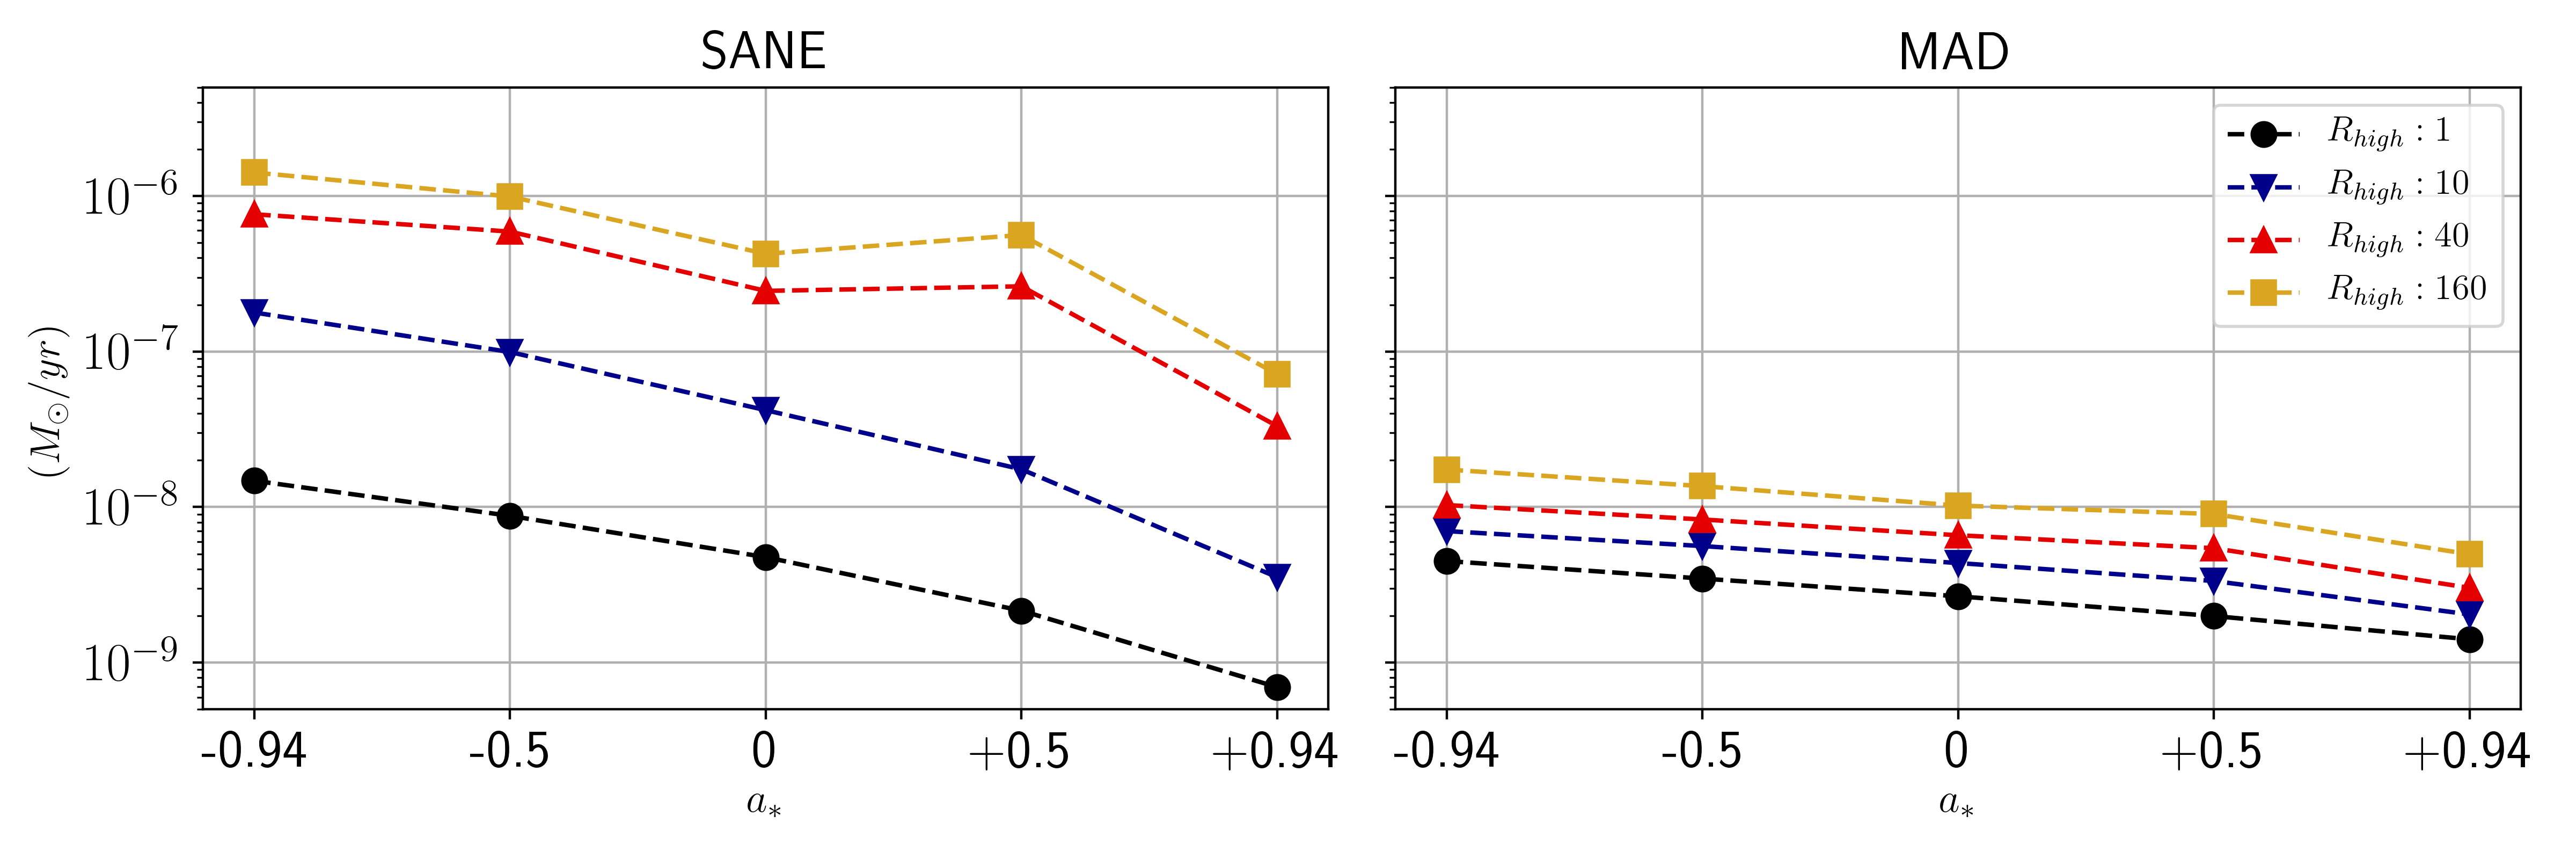
\includegraphics[width=0.95\textwidth]{figures/illinoisv3_average_mdot.png}
\caption{Accretion rate for Illinois-Thermal models}
\label{fig:accretion_illinois_thermal}
\end{figure*}

\begin{figure*}
\centering
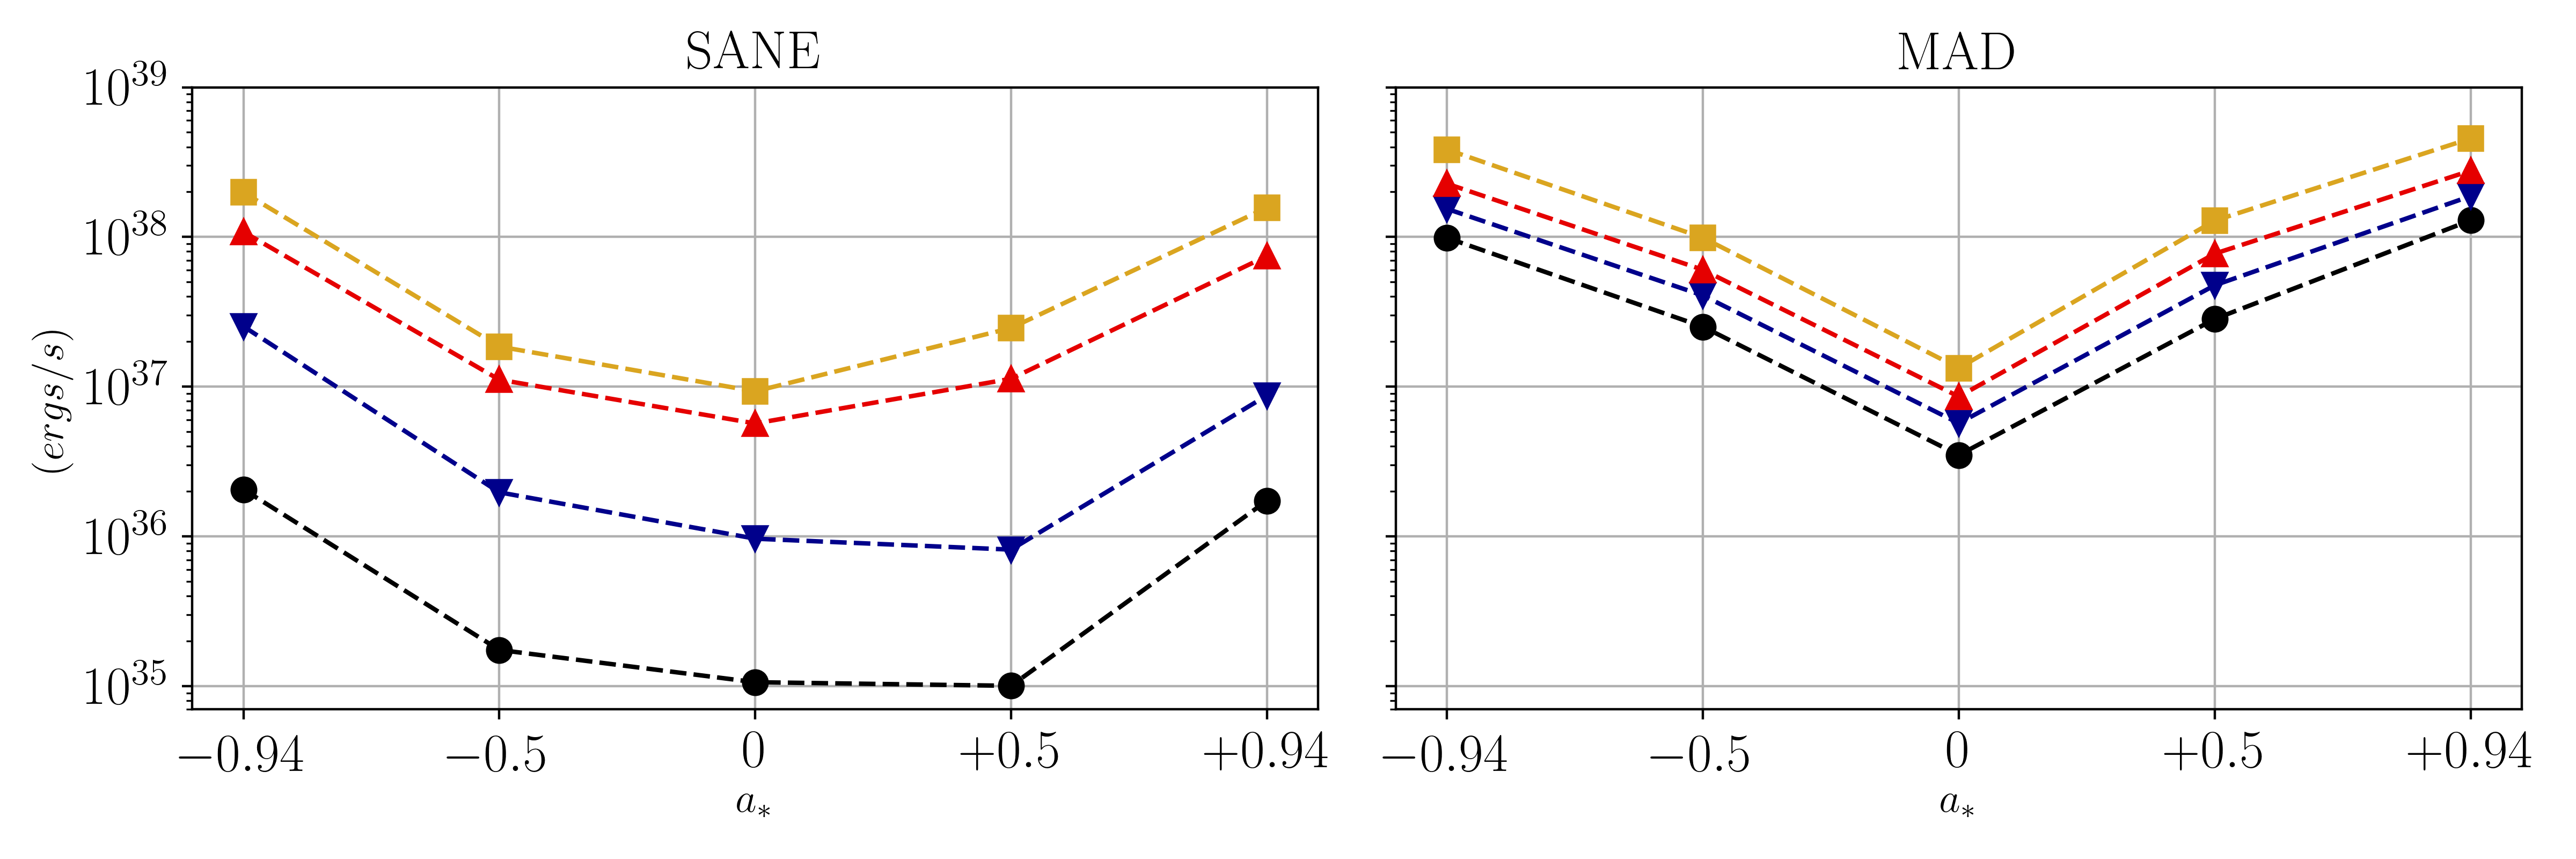
\includegraphics[width=0.95\textwidth]{figures/illinoisv3_average_outflow_power.png}
\caption{Outflow power for Illinois-Thermal models}
\label{fig:outflow_illinois_thermal}
\end{figure*}

Figure showing accretion rate.

Accretion rate is consistent with earlier analyses.

Models at the highest accretion rate are ruled out by overproduction of x-ray emission.  If our models were in equilibrium over a larger range in radius, bremss from larger radius might increase the x-ray flux and rule out more models.

Figure showing outflow power.

Jet power is surprisingly large.  Where does the power come out in the galactic center?

Dependence on distribution function.

\note{Koushik, Alejandro, Razi}

%==============================================================================
\subsection{Positrons}

\monika{i think this section should start with some general statement why do we want to consider positrons at all.}

\cite{2006MNRAS.367..905B} devised a canonical model of Sgr A* as a  radiatively inefficient accretion flow (RIAF). Semi-analytic RIAF models implementing  this using the general relativistic ray tracer GRTRANS \citep{2016MNRAS.462..115D} can be found in  \cite{2021arXiv210105327E}, where  positrons are included using emission modeling motivated in  \cite{2020ApJ...896...30A}. The Figs. 1-3 %\ref{fig:EmamiRIAF}
models from \cite{2021arXiv210105327E} shows Stokes maps and polarized spectra of a \cite{2006MNRAS.367..905B} RIAF with plasma $\beta=10$ and 1$\%$ of the emitting particles nonthermal electrons. The near-extremal ($a/M=0.998$) model shown exhibits Doppler boosting asymmetry in a crescent-shaped intensity pattern with a spiral global electric vector polarization angle (EVPA) pattern and polarization preferentially distributed within this region.

\hyp{As phenomenological models are not considered in this work, the position effect in this subsection may rewrite in a way only focus on the resulting effects and its possible impact for the model images. That is, we may consider to skip the previous paragraph.}
The addition of small non-thermal populations of positrons \citep{2020ApJ...896...30A,2021arXiv210105327E} tends to: increase overall intensity in jet regions for fixed electron number density; modify the low-frequency spectral slope; cancel the observed intrinsic circular polarization and enhance circular polarization due to Faraday conversion. The last of these positron effects is particularly apparent when comparing declining tails of x-ray spectra of positron-rich versus positron-poor sources, as seen in \cite{2021arXiv210105327E}.%Fig. \ref{fig:EmamiRIAFSpectra}.

However, positron effects for Sgr A* are severely limited by the compactness \citep{2012MNRAS.424L..26G} due to the low observed luminosity and outflow geometry. In fact \cite{2011ApJ...735....9M} estimate the funnel positron pair density of Sgr A* to be $10^{-8}\mathrm{cm}^{-3}$ (well below the Goldreich-Julien density required to screen plasma electric fields). By contrast, the comparable density for M87 is $10^3\mathrm{cm}^{-3}$.

%\begin{figure}%[H]
%   \plotone{RIAFSgrAPlaneTscl1Pt5e11beta1Pt0e01fpos0Pt0fNTH1Pt0e-02copy.png}
%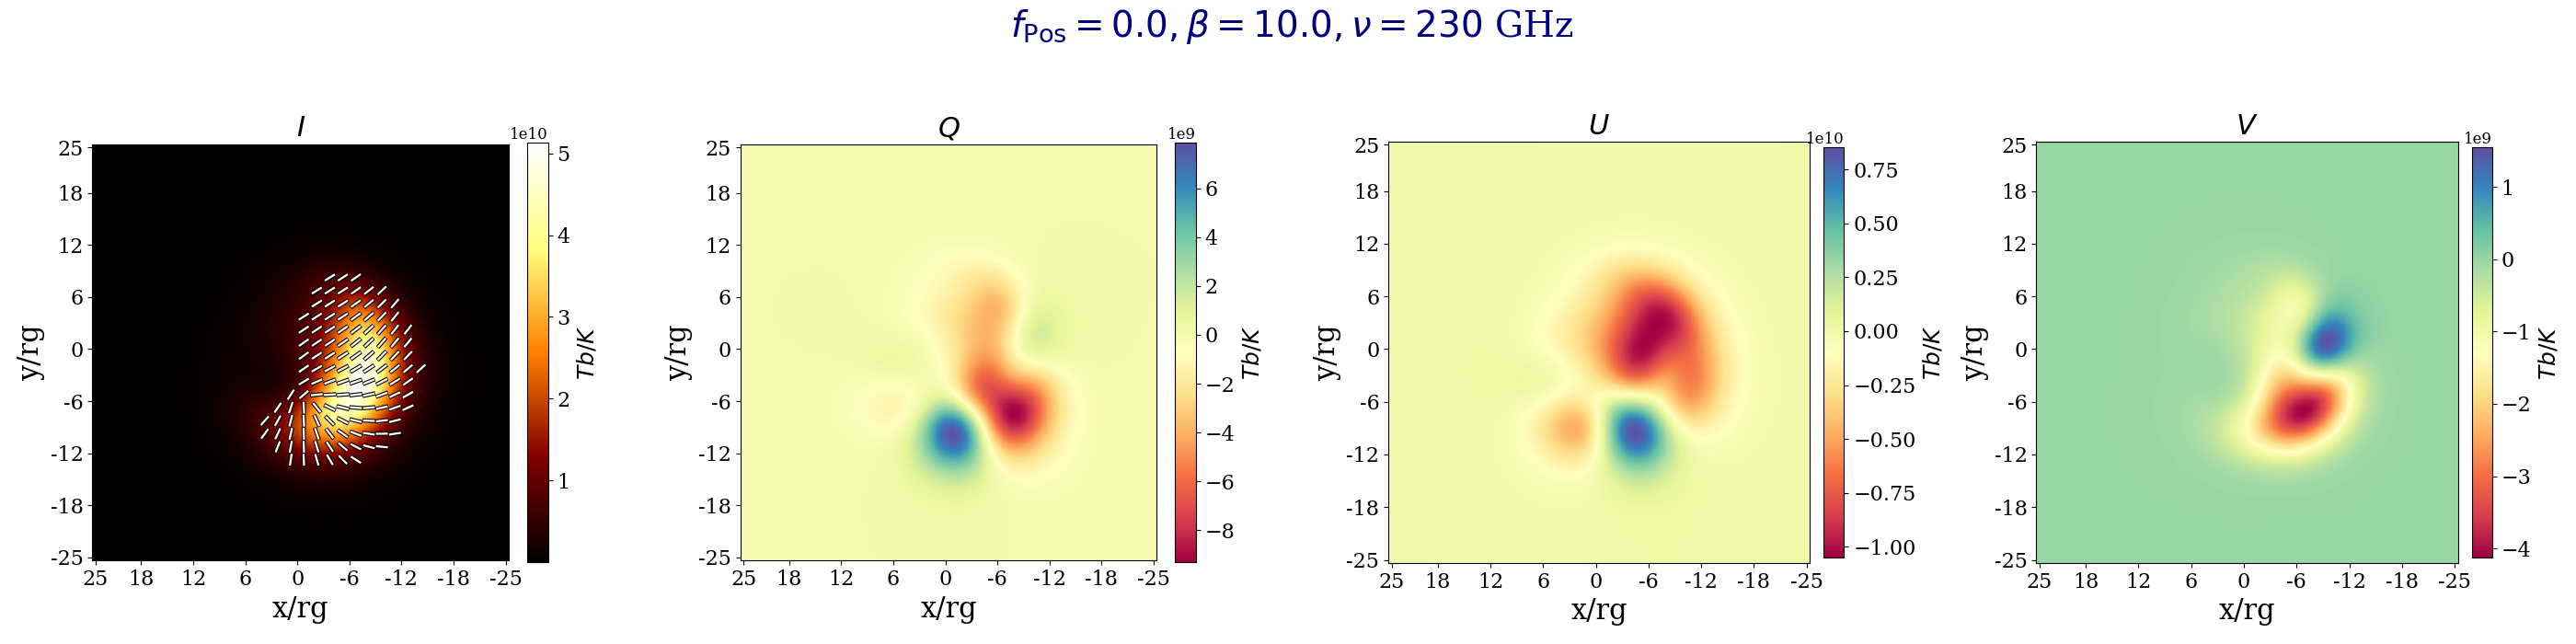
\includegraphics[width=.5\textwidth,height=27mm%,trim=0 380 0 200,clip
%]{RIAFSgrAPlaneTscl1Pt5e11beta1Pt0e01fpos0Pt0fNTH1Pt0e-02copy}
%  \caption{Polarization maps of Stokes parameters $I$, $Q$, $U$ and $V$ at 230 GHz for a \cite{Broderick2005} RIAF with $\beta=10$.}
%  \label{fig:EmamiRIAF}
%\end{figure}

%\begin{figure}%[H]
%\begin{figure*}%[H]
%   \plotone{RIAFSgrAPlaneTscl1Pt5e11beta1Pt0e01fpos0Pt0fNTH1Pt0e-02copy.png}
%  \includegraphics[width=.4\textwidth%width=.55\textwidth,height=25mm%,trim=0 380 0 200,clip
%]{PositronModelEtAl2021RIAFPolSpectra%PolSpectscl1Pt5e11Beta1Pt0e1nth1Pt0em2fpos0Pt0
%}
%  \caption{Polarized SEDs for the Sgr A* RIAF model with  $\beta\in\{10^{-2},10^{0},10^{1}\}$, $f_\mathrm{pos}\in\{0.0,0.5,1.0\}$. The Top Panel shows the Stokes $I$ spectrum, while the Middle Panel shows the SED in linear polarization and the Bottom Panel shows the same for circular polarization.}
%  \label{fig:EmamiRIAFSpectra}
%\end{figure*}
%\end{figure}

%MOVED from Sect. 3.1 to Sect. 3.0
% \textcolor{red}{RJA: Include a summary of analytic/semi-analytic models and Sgr A* simulations in the Literature} Analytic disk $\alpha$-model for angular momentum transport \cite{Shakura1973}. Semi-analytic model motivated in \cite{Yuan2003} and expanded in \cite{Broderick2011}. GRMHD Simulation with hotspots reproducing Sgr A* flares \cite{Ripperda2020}.
%%%%%%%%%%%%%%%%%%%%%%%%%%%%%%%%%%
% \note{to be discussed: how much we would like to discuss polarization emission?}\textcolor{red}{RJA: We should mention the M87 Polarization Collaboration papers \cite{M87PaperVII}, including a comparison of whether Sgr A* is similar enough (e.g., MAD with vertical fields Faraday depolarized on much of the accretion flow) to have an azimuthally spiral EVPA pattern. Figures in  \citep{Emami2021} have similar morphology}.

% \hyp{to-do :  adding historical RIAF fitting result to proto-EHT observations; how recent  GRMHD simulation and subsequent GRRT post-processing suggest other key parameters onto the Broderick 2005 RIAF model; jet componenet? cross referencing MCFE RIAF analysis product?} A proto-EHT array described in \cite{Doeleman2008} estimated the Sgr A* emitting region profile as a circular Gaussian with intrinsic size $37^{+16}_{-10}\ \mu$as.

% % EHT flux vs. baseline observations constrain the emitting region intrinsic size to 37 microarcseconds for a circular Gaussian emission profile

% More recent measurements of closure phases of a few degrees \cite{Fish2016} suggest an asymmetric ring-like profile, with major axis 56 microarcseconds
%%%%%%%%%%%%%%%%%%%%%%%%%%%%%%%%%%
%==============================================================================
\subsection{Caveats and Limitations}\label{sec:limits}

{The mean free path to collisions for particles is typically larger than or comparable to the system size for the accretion disk of \sgra, rendering its plasma collisionless. The GRMHD models employed in this work, describe a collisional system, whereas a first-principles modeling of the collisionless plasma requires a fully kinetic treatment. General relativistic (radiative) kinetic simulations are crucial for dynamically probing the electron temperature, effects of non-thermal distribution functions, and pressure anisotropy and their interplay with radiation in collisionless plasma in the accretion disk and jet. While global general relativistic kinetic simulations cannot be performed with full physical separation between microscopic plasma scales (the particle's Larmor radius $r_{\rm L}$, and plasma skin depth $d_{\rm e}$) and macroscopic scales (the gravitational radius $r_{\rm g}$), they can achieve the right hierarchy of scales ($r_{\rm g} \gg d_{\rm e} \gg r_{\rm L}$) for magnetized plasmas \citep{2018A&A...616A.184L,2018ApJ...863L..31C,2019PhRvL.122c5101P,2020PhRvL.124n5101C,2020ApJ...895..121C,2020ApJ...902...80K,2021A&A...650A.163C,2021PhRvL.127e5101B}. Even in GRMHD, it is computationally challenging to resolve plasma heating processes powering the observed radiation in a converged manner. It is currently not yet feasible to resolve dissipation at the smallest scales of the turbulent cascade or the interplay between turbulence and reconnection at a similar level as in local box simulations \citep{2012ApJ...755...50R,2013ApJ...773..118H,2015PhRvL.114f1101H,2016PhRvL.117w5101K,2017PhRvL.118e5103Z,2018PhRvL.121y5101C,2018ApJ...859..149I,2019PhRvL.122e5101Z,2021ApJ...921...87N,2021arXiv211108188C}. However, \citet{2019ApJS..243...26P} and \citet[in prep.]{Olivares_et_al} show that the global accretion dynamics (mass accretion rate, magnetic flux on the horizon, and MRI quality factor) are converging in our simulations. Some aspects of collisionless plasma dynamics can be described with non-ideal effects (e.g., viscosity, resistivity, heat conduction, pressure anisotropy) in GRMHD models for black hole accretion, e.g.,  \cite{2014MNRAS.440L..41B,2015ApJ...810..162C,2016MNRAS.456.1332F,2017ApJ...837...92C,2017MNRAS.470.2240F,2018ApJ...859...28Q,2019ApJS..244...10R,2019ApJ...882....2V,2020ApJ...900..100R,2021PhRvD.104j3028M,2021arXiv211103689N,2021arXiv211105752M}. For example, the first efforts have recently been made with high-resolution global GRMHD simulations to capture heating through magnetic reconnection in the largest current sheets in the system \citep{2020MNRAS.495.1549N,2020ApJ...900..100R,2021MNRAS.508.1241C,2021arXiv210915115R,2021arXiv211103689N}.}

%==============================================================================
\subsection{Future Constraints}\label{sec:future}

\note{Idea should includes
\emph{i}) integrated polarization,
\emph{ii})  resolved polarization,
\emph{iii}) fits to more sophisticated models such as RIAF analytic models, \ckc{I disagree that RIAF are more ``sophisticated''.  I agree that we can run more models with RIAF in principle, nevertheless.}
\emph{iv}) flux variability \ckc{we don't include it but we should in the future.}
\emph{v})  closure phase variability
}

...